\documentclass[11pt]{article}
\usepackage[margin=1in]{geometry}
\usepackage{amsmath,amssymb,amsthm}
\usepackage{graphicx}
\usepackage{float}
\usepackage[hidelinks]{hyperref}
\usepackage{microtype}
\setlength{\emergencystretch}{2em}
\setlength{\intextsep}{6pt}
\setlength{\abovecaptionskip}{4pt}
\graphicspath{{./}{results/kmeans/}}

\newcommand{\mat}[1]{\begin{bmatrix}#1\end{bmatrix}}

\title{CSE 242 -- Assignment 3}
\author{Yi Zhong \\ \texttt{yzhong76@ucsc.edu}}
\date{Fall 2026}

\begin{document}
\maketitle

%======================================================================
\section{Hard-margin linear SVM}

Positive points: $1=(1,1)$, $2=(1,2)$, $3=(2,1)$; negative points:
$4=(0,0)$, $5=(1,0)$, $6=(0,1)$.

\medskip\noindent\textbf{(a)}
\begin{figure}[H]
\centering
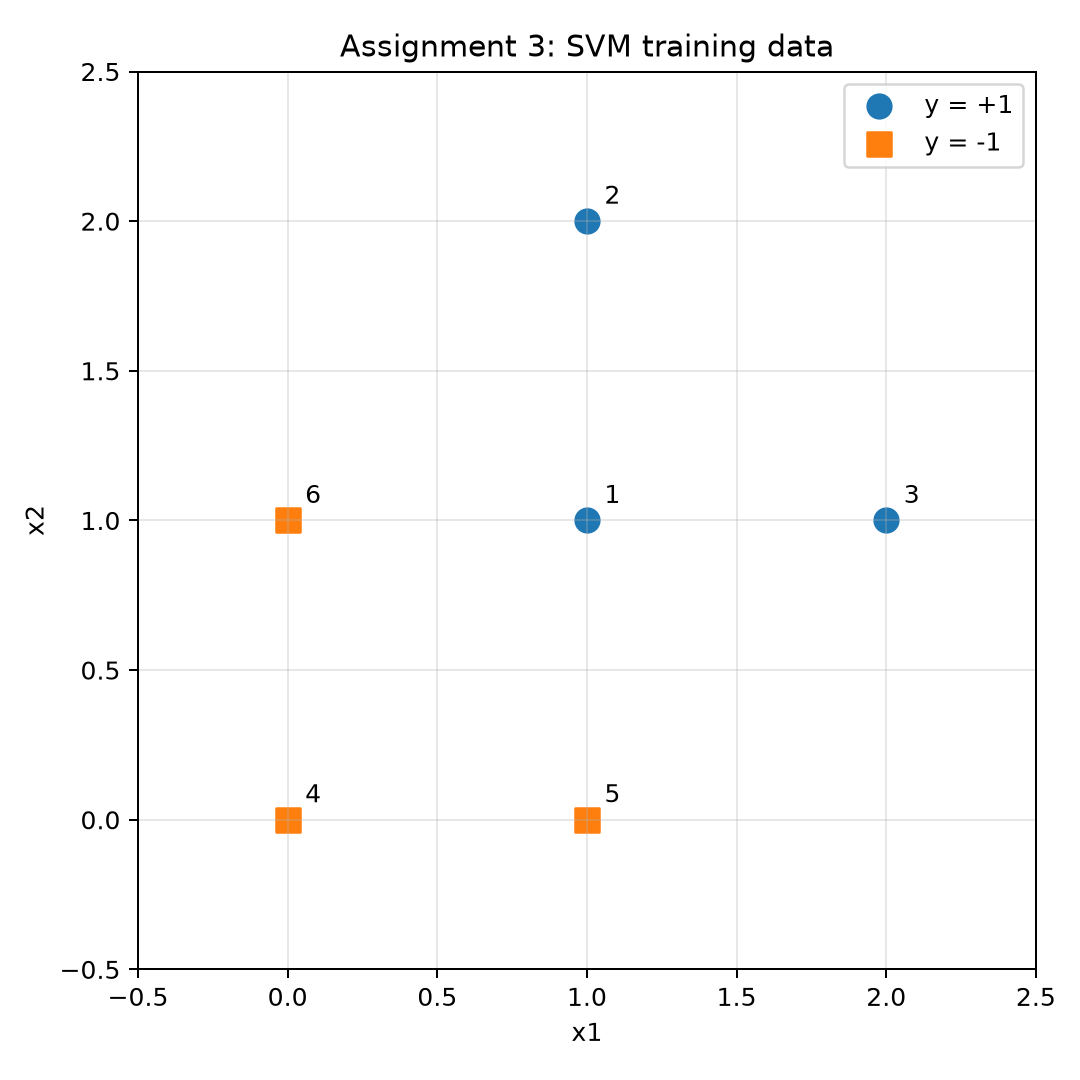
\includegraphics[width=0.4\textwidth]{svm_data.png}
\caption{Training data with point IDs.}
\end{figure}
\noindent Support vectors: points \textbf{1, 5, 6}.
Point 1 lies on $x_1+x_2=2$ and points 5, 6 lie on $x_1+x_2=1$; these are the closest
points of opposite classes, so the widest gap is between these two lines and the boundary
is halfway between them. Points 2, 3 ($x_1+x_2=3$) and 4 ($x_1+x_2=0$) are farther from
the gap.

\medskip\noindent\textbf{(b)}
Each support vector $x_i$ with label $y_i$ lies on its supporting line,
$y_i(w_1x_{i1}+w_2x_{i2}+b)=1$:
\begin{align*}
\text{point 1, } y=+1:&\quad w_1+w_2+b=1\\
\text{point 5, } y=-1:&\quad -(w_1+b)=1 \;\Rightarrow\; w_1+b=-1\\
\text{point 6, } y=-1:&\quad -(w_2+b)=1 \;\Rightarrow\; w_2+b=-1
\end{align*}
Subtracting the second equation from the first gives $w_2=2$, and subtracting the third
from the first gives $w_1=2$; then $b=-1-w_1=-3$:
\[
w=(2,2),\quad b=-3,\qquad \text{boundary } 2x_1+2x_2-3=0\;\;(x_1+x_2=1.5).
\]
Geometric margin (distance from the boundary to the closest points), with
$\|w\|=\sqrt{2^2+2^2}=2\sqrt2$:
\[
\gamma=\frac{|w\cdot x_1+b|}{\|w\|}=\frac{|2+2-3|}{2\sqrt2}=\frac{1}{2\sqrt2}=\frac{\sqrt2}{4}\approx0.354 .
\]

%======================================================================
\section{K-means}

\medskip\noindent\textbf{(a)}
Ties: a point at equal distance from several centroids goes to the one with the smallest
index. Empty clusters: an empty cluster keeps its previous centroid.

\medskip\noindent\textbf{(b)}

\begin{figure}[H]
\centering
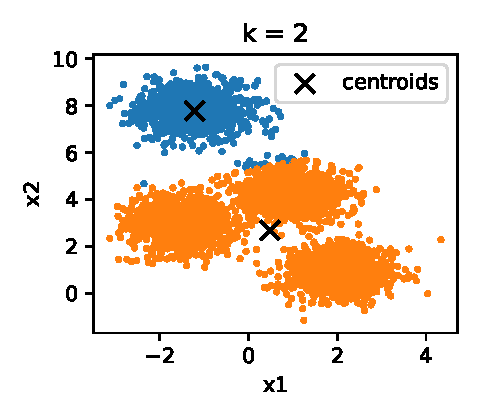
\includegraphics[width=0.32\textwidth]{kmeans_k2.pdf}\hfill
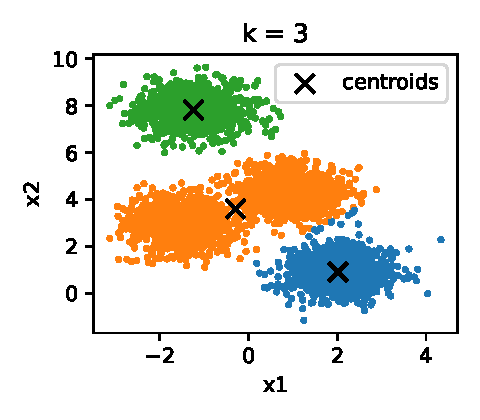
\includegraphics[width=0.32\textwidth]{kmeans_k3.pdf}\hfill
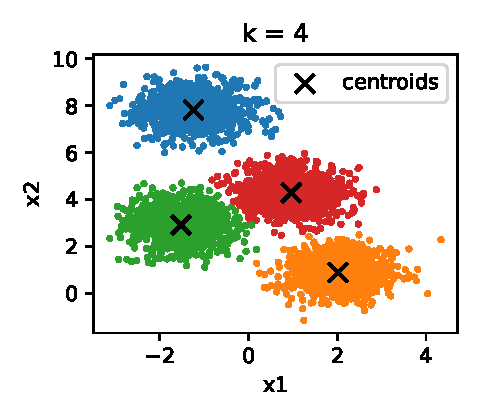
\includegraphics[width=0.32\textwidth]{kmeans_k4.pdf}\\[4pt]
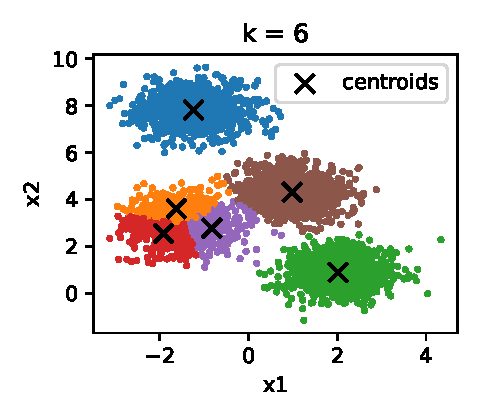
\includegraphics[width=0.32\textwidth]{kmeans_k6.pdf}\quad
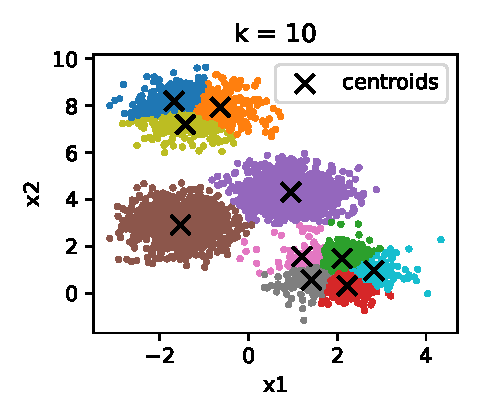
\includegraphics[width=0.32\textwidth]{kmeans_k10.pdf}
\caption{K-means cluster assignments and final centroids for $k=2,3,4,6,10$.}
\end{figure}

With $k=2$ the top group around $(-1.2,7.8)$ forms one cluster and the other three groups
are merged into the second. With $k=3$ the group around $(2.0,0.9)$ separates and the two
middle groups around $(-1.5,2.9)$ and $(1.0,4.3)$ remain merged. With $k=4$ each centroid
lands in one generating group, so the clusters match the four groups. With $k=6$ and
$k=10$ the extra centroids split single groups into pieces, so the clusters become smaller and tighter
but no longer correspond to the generating groups.

%======================================================================
\section{Noisy-label SVM and K-NN repair}

\medskip\noindent\textbf{(a)}
Mean clean-test accuracy over 20 trials (seed 0): \textbf{0.8280}.

\medskip\noindent\begin{minipage}{\textwidth}
\textbf{(b)}
\begin{center}
\begin{tabular}{lc}
\hline
Method & Mean test accuracy (20 trials)\\
\hline
Baseline (noisy labels) & 0.8280\\
K-NN repaired labels & 0.8644\\
\hline
Difference (K-NN $-$ baseline) & $+0.0364$\\
\hline
\end{tabular}
\end{center}
\end{minipage}

\medskip\noindent K-NN repair helped. Positive labels are flipped more often ($0.35$ vs.\ $0.20$), so the
noisy training set has too few positive labels and the baseline SVM predicts $-1$ over
part of the positive region. The positive class is compact (covariance $I$), so most
neighbors of a positive point still have label $+1$ and the vote flips its label back.
Repair can hurt where most neighbors are mislabeled, such as the overlap of the two classes
and the sparse tails of the negative class; there the vote replaces a correct label with a
wrong one.

\end{document}
